% !TeX root=main.tex
\chapter{クイックスタート・ガイド}

本章では,コントローラボードと遠隔サーバのアカウントを入手した人が,コントローラ
ボードを使って回路の動作確認を最初に行うまでの間に必要な手順を説明します.

%%%%%%%%%%%%%%%%%%%%%%%%%%%%%%%%%%%%%%%%%%%%%%%%%%%%%%%%%%%%%%%%%%%%%%%%%%%%%%
\section{アカウントの確認とパスワードの変更}

\textbf{注: 既にパスワードの変更を済ませている場合,本節の作業は不要です.} \vspace*{1ex}

遠隔サーバのアカウントが発行されたら,まずは遠隔サーバにログインできるか確認し,
仮パスワードを自分で決めたパスワードに変更してください.遠隔サーバへのログイン
には PowerShell を使用しますが,PowerShellはデフォルト設定ではフォントの問題で
日本語が文字化けする場合があります.そのため,その対処を行ってから作業すること
をおすすめします.

Windows PowerShell をスタートメニューから開き,タイトルバーを右クリックして,
「プロパティ」を選択します.ダイアログの「フォント」タブから好みの日本語フォ
ントを選択して,OKボタンを押すと,設定が反映されます.

その後,ネットワーク(愛工大の学内環境を使う場合は,学内LAN)に接続されたPCで,
PowerShell から以下のコマンドを入力します.
\begin{verbatim}
    ssh 〈ユーザ名〉@〈接続先〉
\end{verbatim}
ssh のあとには半角スペースが必要であることに注意してください.例えばユーザ名が
\texttt{tu\_fujieda} であり,接続先が \texttt{gw.acri.c.titech.ac.jp}であれば,
入力するコマンドは,
\begin{verbatim}
    ssh tu_fujieda@gw.acri.c.titech.ac.jp
\end{verbatim}
となります.

初回に限り,接続しようとしているサーバの確認を求められるので,yes と入力します.
その後,パスワードの入力を求められるので,発行された仮パスワードを入力します.
このとき文字を入力しても画面上には何の反応もありませんが,それで正常です.

ログインに成功し,画面上に\texttt{〈ユーザ名〉: \$}などといったプロンプトが表示
されたら,\texttt{passwd}(環境によっては\texttt{yppasswd})と入力してパスワード
の変更を行います.
まず仮パスワードを1回入力し,自分で決めたパスワードを2回続けて入力します.
このときもやはり入力内容は画面に反映されませんので,打ち間違いに気をつけてください.
「パスワードは正しく更新されました」,あるいはそれに相当する英語のメッセージが表示
されたら,この段階では PowerShell は閉じても構いません.

%%%%%%%%%%%%%%%%%%%%%%%%%%%%%%%%%%%%%%%
\section{回路設計と必要なファイルの作成}

SawareruSys では,あらかじめ遠隔操作のためのベース設計の回路が用意されています.
ユーザは,その一部を各自で作成した回路に書き換えて使用します.作成した回路を
ベース設計に接続するための回路は,SawareruSys の一部である DRFront を用いて,
自動的に生成します.
回路を作成するためには,作成した回路の各入出力ポートが,FPGA ボードのどの信号に
接続されるかを指定する必要があります.この設定も DRFront の画面上で行います.

まずは配布パッケージの DRFront フォルダにある DRFront.exe 実行ファイルをダブル
クリックして,DRFront を起動します.
デフォルトではハードウェア記述言語(HDL)として VHDL を,FPGA ボードとして
Nexys A7-100T を使用する設定になっていますので,これ以外の言語やボードを使う
場合は,Settings ボタンから使用する言語を変更してください.また,自分の PC に
Vivado をインストールしている場合,インストール先とバージョンを指定すると,
このあとの論理合成と実装までの作業を自分の PC で行えます.
これらの設定は最初の起動時に1回だけ必要です.

作成した回路の HDL 記述を1つのフォルダにまとめておきます.このとき,フォルダ名
に日本語や半角スペースが含まれていると,Vivado の実行時に不具合が発生すること
がありますので,フォルダ名は英数字で作成するようにしてください.自分の PC で
Vivado を動作させる場合,親フォルダについても同様です.

最上段の「Source Dir.」の入力欄の横に「...」と書かれたアイコンがあるので,それを
クリックし,HDL 記述をまとめたフォルダを指定します.記述やディレクトリ名に問題が
なければ,その下の段の「Create Project」というボタンが押せるようになっているので,
このボタンをクリックします.
すると,Projectの項目が「project\_1」に変わり,ボード画像の下のテーブルに,
回路の入出力の一覧が表示されます.このときの様子を図\ref{fig:drfront1_1}に示します.

\begin{figure}[ht]
 \centering
 \fbox{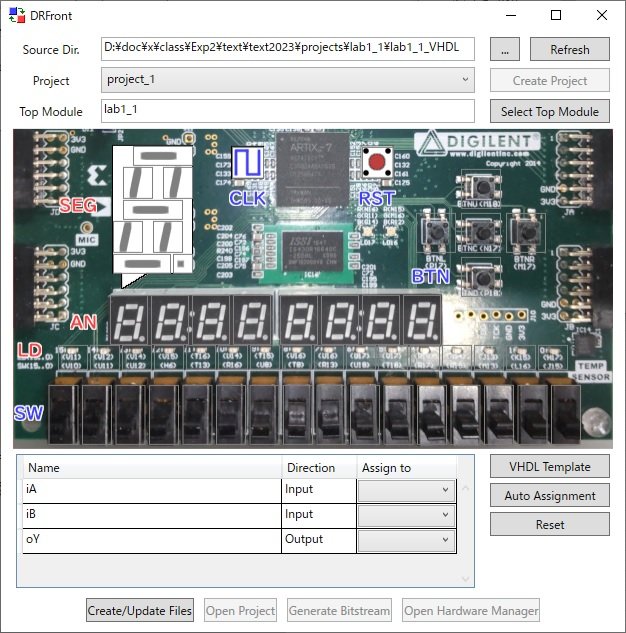
\includegraphics[width=70truemm]{figs/drfront1_1.jpg}}
 \caption{DRFront上でプロジェクトを作成したときの様子.}
 \label{fig:drfront1_1}
\end{figure}

なお,ファイルやディレクトリに問題があり入出力の信号が検出できなかった場合,
「Source Dir.」の入力欄が赤文字で表示されます.また,ディレクトリ名に日本語を
含んでいるなど,後々問題になりうる場合には,入力欄が黄色の背景で表示されます.
いずれもマウスカーソルを当てると問題点が表示されますので,それを参考にファイル
やフォルダ名,保存場所などを適切に修正してください.

入出力の設定には3通りの方法があります.
\begin{enumerate}
 \item 各信号の横の「Assign to」の列から,割当て先の信号を指定する.
 \item 信号名をドラッグして,ボード画像内の割当てたい部品へとドロップする.
 \item 自動割当てを使う.
\end{enumerate}

第1の方法では,「Assign to」の列をクリックすると,割当て可能な信号
(入力であればスイッチやボタン,出力であればLEDなど)の一覧が表示されます.
その中から割当てたい信号名を選ぶと,表の上側のボード画像の対応する部品を
囲む枠が水色で表示されます.これで割当ては完了です.
例として,入力信号iAを右端のスイッチ入力SW(0)に接続したときの様子を
図\ref{fig:drfront1_2}に示します.

\begin{figure}[ht]
 \centering
 \fbox{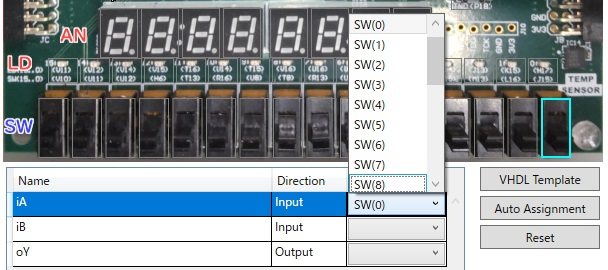
\includegraphics[width=80truemm]{figs/drfront1_2.jpg}}
 \caption{DRFront上で入力信号を割当てたときの様子.}
 \label{fig:drfront1_2}
\end{figure}

第2の方法では,割当てを行いたい信号の行をクリックして選択状態にしたあと,
マウスをドラッグしてボード画像上の割当てたい部品のところへと移動させます.
割当て可能であればマウスカーソルが切り替わり,枠が黄色で表示されるので,
そのままマウスボタンを離します(ドロップします).枠が水色で表示されれば,
割当て完了です.

第3の方法では,表の右側にある「Auto Assignment」ボタンをクリックします.
この方法では,まだ割当てが行われていない信号に対して,入力ならば
SW(0), SW(1), ... が,出力ならば LD(0), LD(1), ... を信号名の順に割当てます.
いくつかの信号を手動で割当てたあとで,自動割当てを行うこともできます.
各自の好みの方法で信号の割当てを行ってください.

すべての入出力への割当てが完了したら,DRFront の左下の「Create/Update Files」
ボタンを押します.すると,Vivadoの実行に必要なファイルが生成された旨が表示
され,「Open Project」ボタンが押せるようになります.

%%%%%%%%%%%%%%%%%%%%%%%%%%%%%%%%%%%%%%%
\section{必要なファイルの転送}

\textbf{注: 自分の PC に Vivado をインストールしている場合,先に2.6節の
「回路の論理合成と実装」の作業を行ってください.} \vspace*{1ex}

DRFront で必要なファイルが生成できたら,WinSCP を使ってそれらを遠隔サーバに
転送します.WinSCP を起動すると,セッション設定画面が表示されます.
転送プロトコルには SFTP または SCP,ホスト名には接続先のホスト名
またはIPアドレス,ユーザ名には遠隔サーバのユーザ名を入力します.
その後,必要に応じて保存ボタンで設定を保存してから,ログインボタンを押します.
SSH の場合と同様,ここでも最初に1回だけサーバの確認があるので,Yesと回答します.
パスワードの入力画面でパスワードを入力して,ログインしてください.

WinSCP のログイン後の画面では,通常左半分に自分のPCのファイル,
右半分に遠隔サーバ上のファイルが一覧表示されます.
ただし設定によっては,遠隔サーバ上のファイルのみが一覧表示される場合もあります.

まずは,遠隔サーバ上の適当な場所にフォルダを作成します.
このとき,Desktop フォルダ上で行うと,あとでリモートデスクトップ接続したときに
デスクトップにフォルダが表示されるので,見つけやすくなるかもしれません.
右半分の画面の適当な空欄を右クリックし,「新規」→「ディレクトリ」でフォルダ
を作成します.
次に,HDL 記述のあるフォルダを WinSCP の左半分の画面か,エクスプローラで開きます. 
フォルダ内にあるすべてのファイルとフォルダをドラッグし,WinSCP の右半分の画面上で
作成したフォルダにドロップすると,ファイル一式が転送されます.

ACRi ルーム上で初めてコントローラボードを使う場合には,2.9節で使用する Connector
アプリ(サーバ)も,このとき遠隔サーバに転送しておきます.配布パッケージの
Connector/Server フォルダにある connector\_serv.py を,遠隔サーバの適当な場所に
転送してください.愛工大の学内環境を使う場合はこの作業は不要です.

この時点で WinSCP は閉じても構いません.もし Vivado 実行後のプロジェクトを自分の
PC にダウンロードしたければ,WinSCP を開いたまま次の作業に進むこともできます.
遠隔サーバ上のファイル一覧は自動では更新されないので,Vivadoを実行するなどして
ファイルが更新されたと考えられる場合には,手動で更新ボタンを押してください.

また,自分のPC上のファイルと遠隔サーバ上のファイルは,自動では同期しないことにも
注意してください.もし記述ミスを見つけるなどして,自分のPC上のファイルを変更した
のであれば,そのファイルは忘れずに遠隔サーバにアップロードしてください.逆に,
遠隔サーバ上のリモートデスクトップでファイルを変更した際には,そのファイルを
遠隔サーバからダウンロードするのも忘れないでください.

ここまでの作業は,開発サーバを予約せずに進めることができます.
そのため,予約した時間が来るまでにここまでの作業を済ませておくと,動作確認が
円滑に進められるでしょう.

%%%%%%%%%%%%%%%%%%%%%%%%%%%%%%%%%%%%
\section{遠隔サーバへの接続}

予約した時間帯になったら,PowerShellを開き,sshコマンドを以下のとおり実行します.
\begin{verbatim}
    ssh -L 13389:〈サーバ名〉:3389 -L 13399:〈サーバ名〉:3399〈ユーザ名〉@〈接続先〉
\end{verbatim}
ただし,サーバ名は予約したサーバの名前,つまり vs + 数字3桁(ACRi ルーム),
または ns + 数字1桁(愛工大の学内環境)となります.
パスワードの入力を求められるので,遠隔サーバのパスワードを入力してログインします.
これにより,ゲートウェイサーバに接続するとともに,開発サーバへのポートフォワー
ディングの設定が行われます.

ログインが完了したら,リモートデスクトップ接続やコントローラボードの接続をして
いる間は PowerShell は開いたままにしておいてください.PowerShell を閉じると,
ポートフォワーディングの設定が解除されるため,リモートデスクトップやコントローラ
ボードも同時に切断されます.

毎回これを打ち込むのが面倒な場合には,上記のコマンドをメモ帳などに書き入れて,
拡張子 .ps1 で保存します.そのファイルを右クリックし「PowerShellで開く」を選択
すれば,自動でコマンドが実行されます.ただし,.ps1 ファイルを実行できない設定に
なっている場合は,以下のコマンドを PowerShell で実行して,実行可能な設定に変更
してください.
\begin{verbatim}
    Set-ExecutionPolicy RemoteSigned -Scope CurrentUser -Force
\end{verbatim}
なお,自分で作成したものでない .ps1 ファイルを安易に実行することはセキュリティ
リスクになりますので,十分注意してください.

%%%%%%%%%%%%%%%%%%%%%%%%%%%%%%%%%%%%
\section{リモートデスクトップ接続と Vivado の起動}

開発サーバ上で Vivado を実行したい場合には,Windows 標準のリモートデスクトップ
接続アプリケーションを使います.スタートメニューの「Windows アクセサリ」から
リモートデスクトップ接続を起動します.起動画面で「オプションの表示」をクリックし,
必要に応じて「画面」タブで画面サイズの設定を行ってください.「全般」タブで
「コンピューター」の欄に\texttt{localhost:13389}と入力して,「接続」ボタンを
押します.初回のみ「このリモートコンピュータのIDを識別できません」という
ウインドウが表示されるので,「このコンピュータへの接続について今後確認しない」を
チェックして,「はい」ボタンを押してください.

\begin{figure}[ht]
 \centering
 \fbox{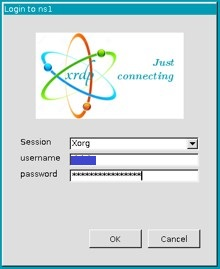
\includegraphics[width=60truemm]{figs/rdp_login.jpg}}
 \caption{開発サーバのログイン画面.}
 \label{fig:rdp_login}
\end{figure}

リモートデスクトップの画面では,最初に図\ref{fig:rdp_login}に示すログイン画面が
表示されます(ACRi ルームではユーザ名は自動入力されます).遠隔サーバのユーザ名
とパスワードを入力してログインします.正しくログインできれば,Ubuntu のデスク
トップ画面が表示されます.
デスクトップ画面が表示されたら,Ctrl+Alt+T キーを押すとターミナルが開きます.
開いたターミナル画面で以下のコマンドを入力すると,Vivado が起動します.
\begin{verbatim}
    source /tools/Xilinx/Vivado/2020.2/settings64.sh
    vivado &
\end{verbatim}
ただし,2020.2 のところは使いたいバージョンに合わせてください.愛工大の学内環境
では,この作業のかわりに,デスクトップに用意されたスクリプト start-vivado.sh を
ダブルクリックすることでも Vivado を起動できます.

%%%%%%%%%%%%%%%%%%%%%%%%%%%%%%%%%%%%
\section{回路の論理合成と実装}

本節の手順で,作成した回路をベース設計の回路と組み合わせて合成し,FPGA に書き込む
ビットストリームファイルを作成します.この作業は標準的には開発サーバ上の Vivado を
用いて行いますが,自分の PC に Vivado がインストールされている場合は,そこで作業
することもできます.

開発サーバ上の Vivado を用いる場合は,Vivado を起動したあと,必要な手順に対応する
スクリプトを読み込ませます.Vivado のメニューの「Tools」→「Run Tcl Script...」を
クリックし,プロジェクトのフォルダ(ソースのあるフォルダの直下に作成されている)
の中にある拡張子 .tcl のファイルを選択します.
自分の PC にインストールされた Vivado を用いる場合は,必要な手順に対応する DRFront
のボタンを押し,DRFront から Vivado を起動します.

\subsection{作成した回路の論理合成}

まずは,作成した回路そのものを論理合成します.開発サーバ上では,OpenProject.tcl を
読み込ませます.自分の PC では,DRFront の「Open Project」ボタンを押します.
10~20秒ほどすると,VHDLファイルのチェックが完了し,回路の階層関係が画面右上の
Sources タブに表示されます.Design Sources の下にあるDR\_TOPが,DRFront によって
作成されたベース設計との接続用の回路です.その横の「>」をクリックすると,この回路
に含まれる回路も表示されます.

階層関係の一例を,図\ref{fig:Vivado1_7_mod}に示します.この図は,DR\_TOP の中に
Deeds-DcSで作成した回路lab1\_1があり,さらにその回路がANDゲート(AND2\_gate)を
使用していることを示しています.

\begin{figure}[ht]
 \centering
 \fbox{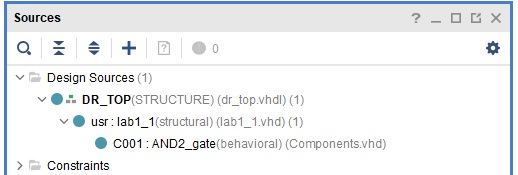
\includegraphics[width=80truemm]{figs/Vivado1_7_mod.jpg}}
 \caption{回路の階層関係表示の例.}
 \label{fig:Vivado1_7_mod}
\end{figure}

回路が無事認識されていることを確認したら,論理合成を行います.メニューの「Flow」
→「Run Synthesis」,または画面左側 Flow Navigator の「SYNTHESIS」→「Run
Synthesis」をクリックします.設定によっては論理合成の設定ダイアログが表示されま
すが,そのままOKボタンを押してください.数十秒ほど待つと論理合成が終了し,
図\ref{fig:Vivado1_8}で示すダイアログが表示されます.ここでは,Open Synthesized
Design を選択して OK ボタンを押し,論理合成結果を確認する画面を開いてください.

\begin{figure}[ht]
 \centering
 \fbox{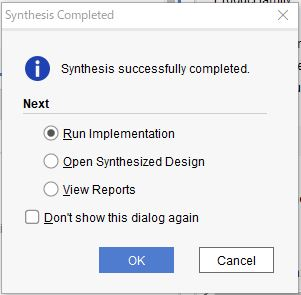
\includegraphics[width=60truemm]{figs/Vivado1_8.jpg}}
 \caption{論理合成成功のダイアログ.}
 \label{fig:Vivado1_8}
\end{figure}

なお,ダイアログを閉じてしまった場合や,論理合成結果を後から確認する必要がある
場合には,メニューの「Flow」→「Open Synthesized Design」または Flow Navigator
の「SYNTHESIS」→「Open Synthesized Design」をクリックすると,この画面に戻って
くることができます.

最後に,論理合成の結果をチェックポイントファイルとして保存します.メニューの
「File」→「Checkpoint」→「Write」から「Write Checkpoint」のダイアログを開き,
ファイル名を変更せずに OK を押します.自分の PC から Vivado を使用している場合,
この時点で Vivado は一旦閉じてしまっても構いません.開発サーバ上の Vivado では,
次のスクリプトを読み込ませると現在の作業内容は自動的に閉じられますので,Vivado
は開いたままで構いません.

\subsection{ベース設計との統合と実装}

ここから行う作業は,ベース設計に先ほど作成した回路を組込み,配置配線を行い,
ビットストリームとよばれるFPGAに書き込むためのデータファイルの作成を行う,
というものです.これらの一連の作業はすべてスクリプトで自動的に実行されます.

開発サーバ上では,GenerateBitStream.tcl を読み込ませます.自分の PC では,
DRFront の「Generate BitStream」ボタンを押します.すべての作業が終了するまでに
1~2分程度かかります.もしも途中でエラーが発生した場合には,Vivado はエラーの
内容を表示して停止します.問題なく全ての手順が完了した場合には,Vivado は
自動的に閉じ(あるいは起動直後の状態に戻り)ます.

本節で自分の PC を使って作業をしていた場合,ここで2.3節に戻り,必要なファイル
の転送とリモートデスクトップ上での Vivado の起動を行うことになります.次の手順
のために最低限転送する必要のあるファイルは,プロジェクトのフォルダの中にある
OpenHW.tcl と (回路名)\_(プロジェクト名).bit の2つのファイルです.

%%%%%%%%%%%%%%%%%%%%%%%%%%%%%%%%%%%%
\section{FPGA への書き込み}

FPGAに書き込むためのビットストリームファイルは,プロジェクトのフォルダの中に,
(回路名)\_(プロジェクト名).bit という名前で用意されます.動作試験前の最後の
手順は,FPGAへこのファイルを書き込むことです.開発サーバ上で起動している Vivado
に OpenHW.tcl を読み込ませます.Vivado が Hardware Manager 画面に切り替わります.
Hardware Manager では,図\ref{fig:Vivado1_12} に示す,まだハードウェアを開いて
いないという旨のメッセージが表示されます.

\begin{figure}[ht]
 \centering
 \fbox{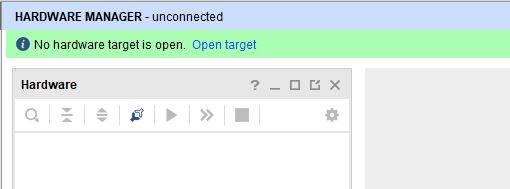
\includegraphics[width=70truemm]{figs/Vivado1_12.jpg}}
 \caption{Hardware Manager画面.}
 \label{fig:Vivado1_12}
\end{figure}

メッセージの横にある Open target のリンクをクリックし,Auto Connect を選択して,
サーバと FPGA との間の接続を行います.正しく接続できていれば,左上の Hardware
タブに (チップ名)\_0 というデバイスが表示され,画面が図\ref{fig:Vivado1_14} 
に示す通りに切り替わります.チップ名には,例えば xc7a100t などといった文字列が
入ります.

\begin{figure}[H]
 \centering
 \fbox{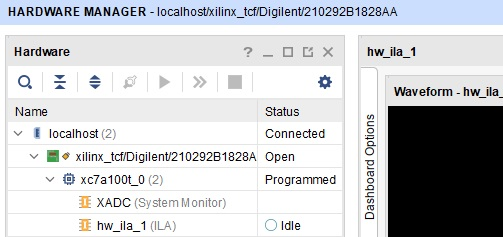
\includegraphics[width=70truemm]{figs/Vivado1_14.jpg}}
 \caption{Hardware ManagerでFPGAが認識されているときの様子.}
 \label{fig:Vivado1_14}
\end{figure}

(チップ名)\_0 を右クリックし,出てきたメニューから Program Device をクリック
すると,書き込むファイルを選択するダイアログが表示されます.「Bitstream file」
の入力欄の横にある「...」ボタンをクリックすると,図\ref{fig:Vivado1_15}に示す
ファイル指定のダイアログが表示されます.

\begin{figure}[H]
 \centering
 \fbox{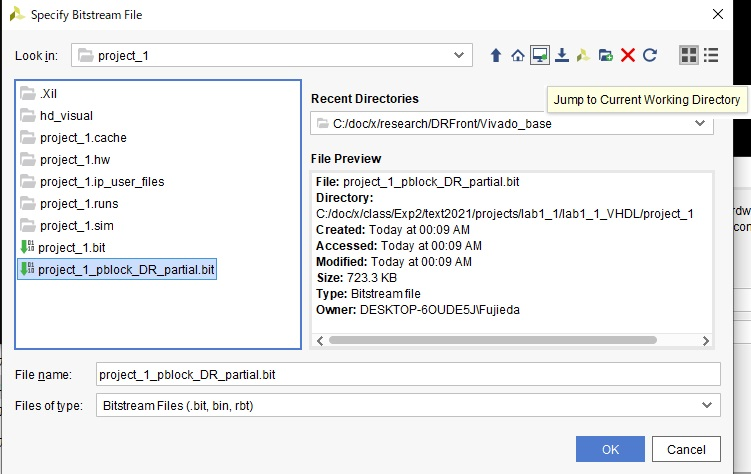
\includegraphics[width=70truemm]{figs/Vivado1_15.jpg}}
 \caption{書き込むビットストリームの選択画面.}
 \label{fig:Vivado1_15}
\end{figure}

ダイアログの右上の
\includegraphics[height=5truemm]{figs/Vivadoicon1_1.png}
のアイコンをクリックするとプロジェクトのディレクトリに移動します.そうすると,
書き込むべき .bit ファイルがファイルリストに現れますので,これを選択して OK 
ボタンを押します.最後に Program ボタンを押すと,ビットストリームが FPGA に
書き込まれ,作成した回路が動作を開始します.

ここまで開発サーバ上で Vivado を操作していた場合,Vivado 起動から FPGA への
書き込みまでの間に必要な手順は以下の通りとなります.

\begin{enumerate}
 \item Tool → Run Tcl Script で OpenProject.tcl を実行する
 \item Run Synthesis で論理合成を行う
 \item Open Synthesized Design で合成結果を開く
 \item File → Checkpoint → Write でチェックポイントを保存
 \item Tool → Run Tcl Script で GenerateBitstream.tcl を実行する
 \item Tool → Run Tcl Script で OpenHW.tcl を実行する
 \item Open target → Auto Connect でボードと接続する
 \item (チップ名)\_0 を右クリックして,Program Device を行う
\end{enumerate}

%%%%%%%%%%%%%%%%%%%%%%%%%%%%%%%%%%%%
\section{Connector アプリ(サーバ側)の準備}

\textbf{注: 愛工大の学内環境ではこの作業は不要です.Connector アプリが常時起動
する設定になっています.} \vspace*{1ex}

コントローラボードを使った動作確認のために,コントローラボードと FPGA ボードと
の間の通信を中継する Connector アプリを,サーバ側,PC 側の両方で起動します.
本節ではまずサーバ側の Connector アプリを起動します.

ターミナル上で2.3節で転送した connector\_serv.py のあるフォルダに移動します.
その上で,以下のコマンドで Connector アプリを起動します.
\begin{verbatim}
  python3 connector_serv.py /dev/ttyUSB1 3399
\end{verbatim}

Connector アプリが起動すると,動作ログがターミナル上に表示されます.FPGA
ボードが正しく認識できている場合,動作ログは例えば以下のような内容となります.
\begin{verbatim}
[2024-04-01 13:41:37] Connector for SawareruSys started.
[2024-04-01 13:41:37] Serial port opened.
[2024-04-01 13:41:37] Server started listening.
\end{verbatim}
Connector アプリを終了させたい場合には,Ctrl+C キーを押してください.

%%%%%%%%%%%%%%%%%%%%%%%%%%%%%%%%%%%%
\section{Connector アプリ(PC 側)の準備と動作確認}

つづいて,PC 側でも同様に通信の中継を設定します.PC 側で使用する Connector アプリ
は,配布パッケージの Connector/Client フォルダにある,Connector.exe 実行ファイル
です.

コントローラボードと PC を USB ケーブルで接続したあと,Connector アプリを起動
します.Controller Board の欄の下の None をクリックすると,その時点で接続されて
いるシリアル通信デバイスの一覧が表示されます.通常,コントローラボードは「USB
シリアル デバイス」という名前で認識されますので,その名前のついたデバイスを選択
してください.そうすると,Controller Board の欄下部の表示が,選択したデバイスの
ポート番号(COM + 数字)に切り替わります.FPGA ボード側のポート番号は,通常変更
する必要はありません.2.4節で遠隔サーバに接続したときに設定したポート番号(13399)
が自動で入力されています.Connector アプリでシリアル通信デバイスの一覧が表示
されているときの様子を,図\ref{fig:connector_port}に示します.

\begin{figure}[ht]
 \centering
 \fbox{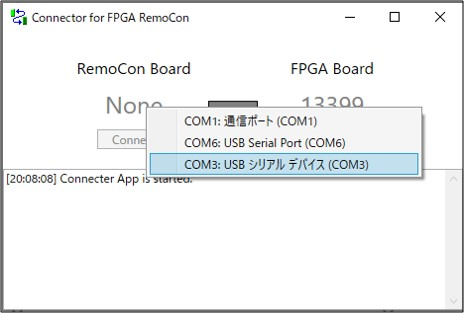
\includegraphics[width=60truemm]{figs/connector_port.jpg}}
 \caption{Connectorアプリのポート設定の例.}
 \label{fig:connector_port}
\end{figure}

ポート設定が済んだら,Connector アプリの両サイドの Connect ボタンを両方クリック
します.ボタン上の文字の色がともに青色に変わり,中央のバーの色が青色に変われば,
手元のコントローラボード,遠隔の FPGA ボードともに正しく認識されています.
この状態になれば,コントローラボードの入力を操作することで,FPGA ボードの入力を
遠隔で操作できるようになっているはずです.また,FPGA ボードの出力が,コントローラ
ボード上の LED や7セグメント LED で確認できるようになっているはずです.

%%%%%%%%%%%%%%%%%%%%%%%%%%%%%%%%%%%%
\section{接続を終了する前に}

動作確認をやめる場合には,まず PC 側の Connector アプリを終了して,コントローラ
ボードに接続された USB ケーブルを抜きます.リモートデスクトップ上では,Vivado と
サーバ側の Connector アプリを終了し,デスクトップ右上の電源マークのアイコンから,
「電源オフ/ログアウト」→「ログアウト」を選択して,開発サーバからログアウトします.

これらを確認してから,PowerShell を閉じて,遠隔サーバとの接続を終了してください.
PowerShell を先に閉じてしまうと,次回以降のログイン時に問題が生じる場合があります.

%%%%%%%%%%%%%%%%%%%%%%%%%%%%%%%%%%%%%%%%%%%%%%%%%%%%%%%%%%%%%%%%%%%%%%%%%%%%%%%